\documentclass[tikz, border=4pt]{standalone}
\usepackage[T1]{fontenc}
\usepackage{lmodern}
\usetikzlibrary{positioning, calc, arrows.meta}

% Typography, palette, card outlines and arrows follow
% fig-evidence-workflow-tikz.tex.
% Two-layered reading strategy and card text follow the rater instructions
% "Evidence Rating Revised_final instructions" (20 November 2026): the former
% proximity-reading step and its keyword panels are dropped; the list of the
% twelve functions is kept without keywords.
\definecolor{leg}{HTML}{2166ac}
\definecolor{irr}{HTML}{b2182b}
\definecolor{band}{HTML}{dbe6f2}
\definecolor{pale}{HTML}{f3f3f3}

\begin{document}
\hyphenpenalty=10000
\exhyphenpenalty=10000
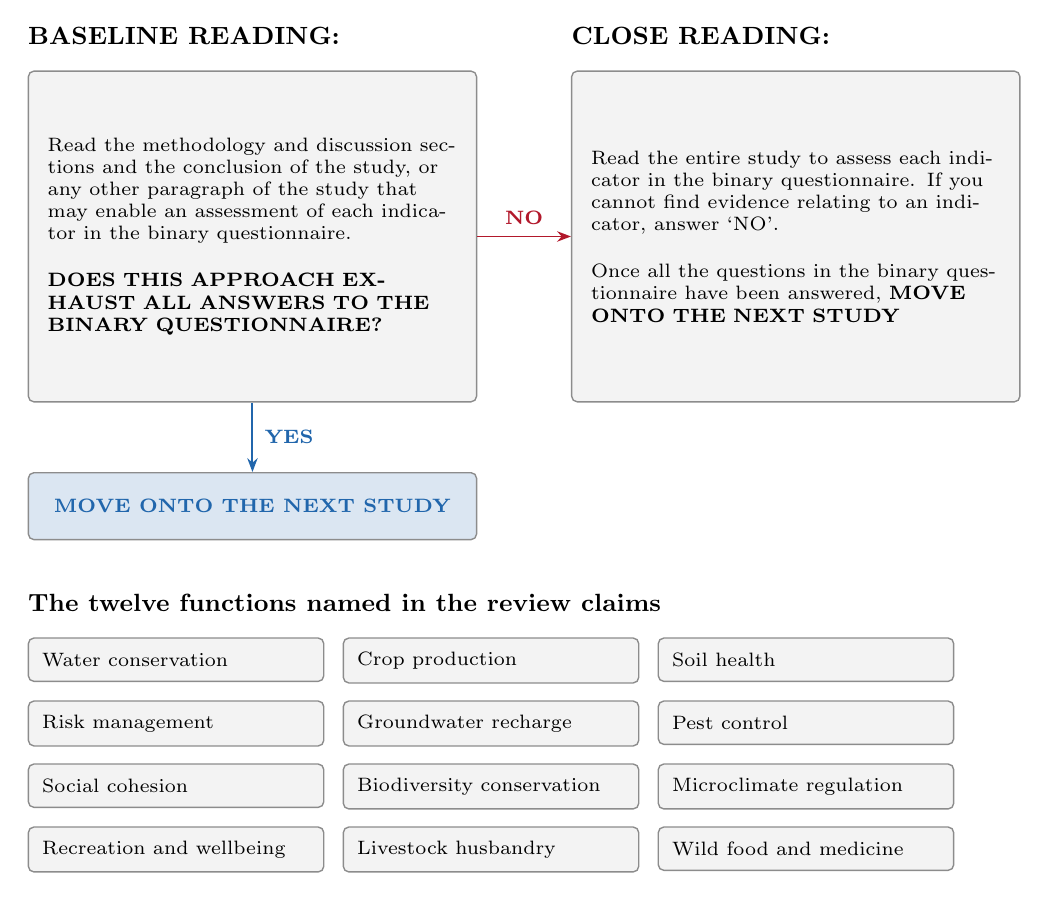
\begin{tikzpicture}[
  font=\footnotesize,
  stp/.style={font=\bfseries\small, anchor=north west, inner sep=0pt},
  card/.style={draw=black!45, fill=pale, rounded corners=2pt,
    line width=0.5pt, inner sep=7pt, align=left, font=\scriptsize,
    text width=5.2cm, minimum height=4.2cm, anchor=north west},
  done/.style={card, fill=band, text=leg, font=\scriptsize\bfseries,
    align=center, minimum height=0.85cm},
  fun/.style={draw=black!45, fill=pale, rounded corners=2pt,
    line width=0.5pt, inner sep=5pt, align=left, font=\scriptsize,
    text width=3.4cm, minimum height=0.55cm, anchor=north west},
  group/.style={font=\bfseries\footnotesize, anchor=north west, inner sep=0pt},
  arr/.style={-{Stealth[length=5pt]}, black!60, line width=0.7pt},
  label/.style={font=\scriptsize\bfseries, fill=white, inner sep=2pt},
]

\node[stp] (h1) at (0,0) {BASELINE READING:};
\node[stp] (h2) at (6.9,0) {CLOSE READING:};

\node[card] (baseline) at (0,-0.55) {%
  Read the methodology and discussion sections and the conclusion of the
  study, or any other paragraph of the study that may enable an assessment
  of each indicator in the binary questionnaire.
  \par\vspace{9pt}
  \textbf{DOES THIS APPROACH EXHAUST ALL ANSWERS TO THE BINARY QUESTIONNAIRE?}
};

\node[card] (close) at (6.9,-0.55) {%
  Read the entire study to assess each indicator in the binary
  questionnaire. If you cannot find evidence relating to an indicator,
  answer `NO'.
  \par\vspace{9pt}
  Once all the questions in the binary questionnaire have been answered,
  \textbf{MOVE ONTO THE NEXT STUDY}
};

\node[done] (next1) at (0,-5.65) {MOVE ONTO THE NEXT STUDY};

\draw[arr, draw=irr] (baseline.east) -- node[label, text=irr, above=2pt] {NO} (close.west);
\draw[arr, draw=leg] (baseline.south) -- node[label, text=leg, right=2pt] {YES} (next1.north);

% The twelve functions served by traditional irrigation
\node[stp] at (0,-7.2) {The twelve functions named in the review claims};
\foreach \i/\name in {0/Water conservation, 1/Crop production, 2/Soil health,
                      3/Risk management, 4/Groundwater recharge, 5/Pest control,
                      6/Social cohesion, 7/Biodiversity conservation, 8/Microclimate regulation,
                      9/Recreation and wellbeing, 10/Livestock husbandry, 11/Wild food and medicine} {
  \pgfmathtruncatemacro{\col}{mod(\i, 3)}
  \pgfmathtruncatemacro{\row}{int(\i / 3)}
  \node[fun] at ({\col*4.0}, {-7.75 - \row*0.8}) {\name};
}

\end{tikzpicture}
\end{document}
